\section{Seleccionar una medida de desempeño}

El siguiente paso es seleccionar una medida de desempeño. Una forma típica de medir para problemas de regresión es el error de la raíz media cuadrática (RMSE). Este nos da una idea cómo el error del sistema típicamente hace en sus predicciones, con un alto peso para errores grandes. La ecuación~\eqref{eq:rmse}
\begin{equation}\label{eq:rmse}
\operatorname{RMSE}\left(\bm{X},h\right)=\sqrt{\frac{1}{m}\sum_{i=1}^{m}{\left(h\left(\bm{x}^{\left((i)\right)}\right)-y^{\left(i\right)}\right)}^{2}}
\end{equation}
\begin{itemize}
	\item $m$ es el número de instancias en el conjunto de datos que se está midiendo.
	\item $\bm{x}^{\left(i\right)}$ es un vector de todos los valores de la característica (excluyendo la etiqueta) de la $i$--ésima instancia en un conjunto de datos, e $y^{\left(i\right)}$ es su etiqueta (el valor deseado de salida para esa instancia).
	\item $\bm{X}$ es una matriz que contiene todos los valores característicos (excluyendo etiquetas) de todas las instancias en un conjunto de datos.
	\item $h$ es la función del sistema predictivo, también llamado \emph{hipótesis}. Cuando el sistema es dado una característica de instancia, su salida es el valor predecido $\hat{y}^{\left(i\right)}=h\left(\bm{x}^{\left(i\right)}\right)$ para la instancia.
	\item $\operatorname{RMSE}\left(\bm{X},h\right)$ es la función de costo medido en un conjunto de ejemplos usando la hipótesis $h$.
\end{itemize}
Incluso pensado que la RMSE es generalmente la medida de desempeño preferido para las tareas de regresión, en algunos contextos podría preferir usar otra función. Por ejemplo, suponga que existen muchos distritos outliers. En este caso, podría considerar usar el \emph{error cuadrático medio} (también llamada la desviación media absoluta, vea la ecuación~\eqref{eq:mae})
\begin{equation}\label{eq:mae}
\operatorname{MAE}\left(\bm{X},h\right)=\frac{1}{m_{i}}\sum_{i=1}^{m}\left|h\left(\bm{x}^{\left(i\right)}.y^{\left(i\right)}\right)\right|
\end{equation}
Tanto la RMSE como la MAE son maneras de medir la distancia entre dos vectores: el vector de predicción y el vector de valores objetivo. Varias medidas de distancias, son posibles:
\begin{itemize}
	\item Calculando la raíz cuadrada de una suma de cuadradas (RMSE) corresponde a la \emph{norma euclidiana}: esta es la noción de distancia con la que está familiarizado. Este es llamado la norma $\ell_{2}$, denotado por $\left\|\cdot\right\|_{2}$ (o solo $\left\|\cdot\right \|$).
	\item Calculando la suma de los valores absolutos (MAE) corresponde a la norma $\ell_{1}$, denotado por $\left\|\cdot\right\|_{1}$. A veces llamada \emph{norma Manhattan} porque este mide la distancia entre dos puntos en una ciudad si solo puede viajar a lo largo de cuadras ortogonales.
	\item Más generalmente, la \emph{norma} $\ell_{k}$ de un vector $\bm{v}$ que contiene $n$ elementos es definido por ${\left({\left|v_{0}\right|}^{k}+{\left|v_{1}\right|}^{k}+\cdots+{\left|v_{n}\right|}^{k}\right)}^{\frac{1}{k}}$. $\ell_{0}$ da el número de elementos no nulos en el vector y $\ell_{\infty}$ da el máximo valor absoluto en el vector.
	\item El mayor índice de la norma, %TODO
	se centra en valores grandes y %TODO
	Este es la razón por la que RMSE es más sensitiva a los outliers que el MAE. Pero cuando
\end{itemize}

En este capítulo, empezaremos mirando un modelo de regresión lineal, uno de los modelos más simple que hay. Discutiremos dos maneras muy diferentes de tratar:
\begin{itemize}
	\item Usando la fórmula cerrada que directamente calcula los parámetros del modelo que minimiza la función de costo sobre el conjunto de datos.
	\item Usando un método de optimización iterativa, llamado el \emph{descenso del gradiente}, que gradualmente ajusta los parámetros para minimizar la función de consto sobre el conjunto de datos, eventualmente convergiendo al mismo conjunto de parámetros como el primer método. Veremos algunas pocas variantes del descenso del gradiente.
\end{itemize}
Luego, veremos la regresión polinomial, un modelo complejo que puede ajustar conjunto de datos no lineales. Dado que este modelo tiene más parámetros que la regresión lineal, este es %TODO
así veremos cómo detectar cuando es o no el caso, usando curvas de aprendizaje, y entonces veremos varias técnicas de regularización que pueden reducir el sobreajuste del conjunto de datos. Finalmente, veremos sobre dos modelos comúnmente usados para tareas de clasificación: la regresión logística y la regresión softmax.

En %TODO la ecuación X, vimos un modelo de regresión lineal de 
Este modelos es solo una función lineal con características de entrada %TODO:
$\theta_{0}$ y $\theta_{1}$ son los parámetros del modelo.

Más generalmente, un modelo lineal hace una predicción por simple cálculo de suma de pesos de características de entrada, más una constante llamada el térmnino intercepto, como se muestra en la ecuación~\eqref{eq:linear}
\begin{equation}\label{eq:linear}
\hat{y}=\theta_{0}+\theta_{1}x_{1}+\theta_{2}x_{2}+\cdots\theta_{n}x_{n}
\end{equation}
\begin{itemize}
	\item $\hat{y}$ es el valor predecido.
	\item $n$ es el número de características.
	\item $\theta_{j}$ es el $j$--ésimo parámetro del modelo (incluyendo el término intercepto $\theta_{0}$ y los pesos de las características $\theta_{1},\theta_{2},\ldots,\theta_{n}$).
\end{itemize}
Esto puede ser escrito mucho más conciso usando una forma vectorial, como se muestra en~\eqref{eq:linearvector}
\begin{equation}\label{eq:linearvector}
\hat{y}=h_{\bm{\theta}}\left(\bm{x}\right)=\bm{\theta}\cdot\bm{x}
\end{equation}
\begin{itemize}
	\item $\bm{\theta}$ es parámetro vector del modelo, conteniendo el término intercepto $\theta_{0}$ y los pesos características desde $\theta_{1}$ hasta $\theta_{n}$.
	\item $\bm{x}$ es la instancia del vector característica, conteniendo desde $x_{0}$ hasta $x_{n}$, con $x_{0}=1$.
	\item $\bm{\theta}\cdot\bm{x}$ es el producto interno de $\bm{\theta}$ y $\bm{x}$, el cual es igual a $\theta_{0}x_{0}+\theta_{1}x_{1}+\cdots\theta_{n}x_{n}$.
	\item $h_{\bm{\theta}}$ es la función de hipótesis, usando los parámetros $\theta$ del modelo.
\end{itemize}

En el apéndice 1
% TODO:
vimos que la forma más compun de medir el desempeño de un modelo de regresión es la raíz cuadrática media (RMSE). Por lo tanto, para emplear el modelo de regresión limeal, necesitarás encontrar el valor de $\bm{\theta}$ que minimice la RMSE. En la práctica, es más simple minimizar el error cuadrático medio (MSE) que el RMSE, y se consigue el mismo resultado (porqe el valor que minimiza una función también minimiza su raíz cuadrada).

El MSE de una hipótesis de regresión lineal $h_{\bm{\theta}}$ en un conjunto de datos $\bm{X}$ es calculado usando la ecuación~\eqref{eq:mse}
\begin{equation}\label{eq:mse}
\operatorname{MSE}\left(\bm{X},h_{\bm{\theta}}\right)=\frac{1}{m_{i}}\sum_{i=1}^{m}{\left(\bm{\theta}^{T}\bm{x}^{\left(i\right)}-y^{\left(i\right)}\right)}^{2}
\end{equation}
La única diferencia es que escribimos $h_{\bm{\theta}}$ en vez de solo $h$ para hacer más claro que el modelo es parametrizado por el vector $\bm{\theta}$. Para simplificar notaciones, solo escribiremos $\operatorname{MSE}\left(\bm{\theta}\right)$ en vez de $\operatorname{MSE}\left(\bm{X},h_{\bm{\theta}}\right)$.

\subsection{La ecuación normal}
Para encontrar el valor de $\bm{\theta}$ que minimice la función de costo, existe una solución en \emph{forma cerrada}, en otras palabras, una ecuación matemática que nos da el resultado directo. Esto es llamado la \emph{ecuación normal}
\begin{equation}
\hat{\bm{\theta}}={\left(\bm{X}^{T}\bm{X}\right)}^{-1}\bm{X}^{T}\bm{y}
\end{equation}
\begin{itemize}
	\item $\hat{\bm{\theta}}$ es el valor de $\bm{\theta}$ que minimiza la función de costo.
	\item $\bm{y}$ es el vector de valores objetivos conteniendo desde $y^{\left(1\right)}$ hasta $y^{\left(m\right)}$.
\end{itemize}
Ahora generemos datos para probar esta ecuación en
\begin{pygments}{pycon}
>>> import numpy as np
>>> X = 2*np.random.rand(100, 1)
>>> y = 4 + 3*X + np.random.randn(100, 1)
\end{pygments}
Ahora calculemos $\hat{\bm{\theta}}$ usando la ecuación normal. Usaremos la función \pygment{python}{inv()} del módulo de álgebra lineal de Numpy (\pygment{python}{np.linalg}) para calcular la inversa de una matriz, y el método \pygment{python}{dot()} para la multiplicación de matrices:
\begin{pygments}{pycon}
>>> X_b = np.c_[np.ones((100, 1)), X] # Sumar x0 = 1 para cada instancia
>>> theta_best = np.linalg.inv(X_b.T.dot(X_b)).dot(X_b.T).dot(y)
\end{pygments}
La función actual usaremos para generar este dato es $y=4+3x_{1}+\text{Ruido gaussiano}$. Vemos que la ecuación encontrada:
\begin{pygments}{pycon}
>>> theta_best
array([[4.22606177],
[2.92965516]])
\end{pygments}
Podríamos esperar para $\theta_{0}=4$ y $\theta_{1}=3$ en vez de $\theta_{0}=4.215$ y $\theta_{1}=2.770$. Muy cercano, pero el ruido hace imposible recuperar los parámetros exactos de la función original.

Ahora puede hacer predicciones usando $\hat{\bm{\theta}}$:
\begin{pygments}{pycon}
>>> X_new = np.array([[0], [2]])
>>> X_new_b = np.c_[np.ones((2, 1)), X_new] # Suma x0=1 en cada instancia
>>> y_predict = X_new_b.dot(theta_best)
>>> y_predict
array([[ 3.86893532],
[10.18025405]])
\end{pygments}
Ahora grafiquemos los modelos de predicciones ():
\begin{pylabcode}[plotsession]
rc('text', usetex=True)
rc('font', **{'family':'serif', 'serif':['Times']})
rc('legend', fontsize=10.0)
X = 2*rand(100, 1)
y = 4 + 3*X + randn(100, 1)
X_b = np.c_[ones((100, 1)), X]
theta_best = linalg.inv(X_b.T.dot(X_b)).dot(X_b.T).dot(y)
X_new = array([[0], [2]])
X_new_b = c_[np.ones((2, 1)), X_new]
y_predict = X_new_b.dot(theta_best)
y_predict
plot(X_new, y_predict, 'r--',X, y, 'b.')
plot(X, y, "b.")
axis([0, 2, 0, 15])
savefig('plot.pdf', bbox_inches='tight')
\end{pylabcode}
%\begin{figure}[ht!]
%	\centering
%	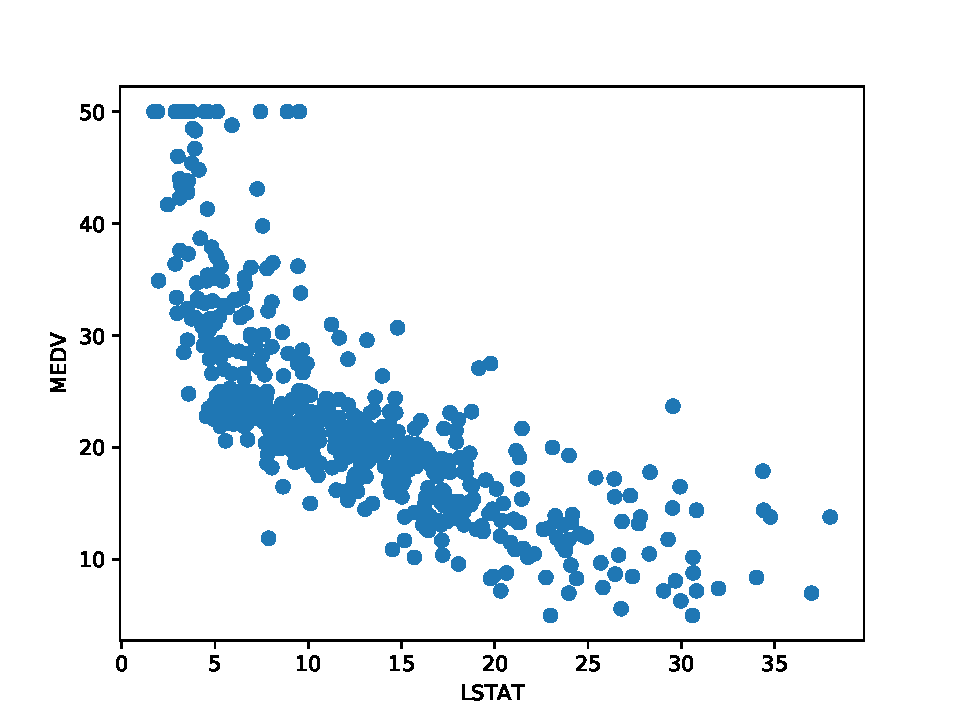
\includegraphics[width=0.4\paperwidth]{plot}
%	\caption{\label{fig:plottheta}Recta de regresión}
%\end{figure}
Mejoramos la regresión lineal usando Scikit-Learn es un poco simple:
\begin{pygments}{pycon}
>>> from sklearn.linear_model import LinearRegression
>>> lin_reg = LinearRegression()
>>> lin_reg.fit(X, y)
>>> lin_reg.intercept_, lin_reg.coef_
(array([4.21509616]), array([[2.77011339]]))
>>> lin_reg.intercept_, lin_reg.coef__
array([[4.2150916], [9.75532293]])
\end{pygments}
La clase \pygment{python}{LinearRegression} está basado en la función \pygment{python}{scipy.linalg.lstsq()} (el nombre abreviado de ``mínimos cuadrados''), el cual puede llamarlo directamente:
\begin{pygments}{pycon}
>>> theta_best_svd, residuals, rank, s = np.linalg.lstsq(X_b, y, rcond=1e-6)
>>> theta_best_svd
array([[4.21509616], [2.77011339]])
\end{pygments}
La función calcula $\hat{\bm{\theta}}=\bm{X}^{+}\bm{y}$, donde $\bm{X}^{+}$ es la \emph{pseudoinversa} de $\bm{X}$ (específicamente la inversa de Moore-Penrose). Puede usar \pygment{python}{np.linalg.pinv()} para calcular la pseudoinversa directamente:
\begin{pygments}{pycon}
>>> np.linalg.pinv(X_b).dot(y)
array([[4.21509]])
\end{pygments}
La pseudoinversa por sí misma es calculada usando la técnica estándar de factorización de matrices llamada la \emph{descomposición de valores singulares} que puede ser descompuesta la matriz $\bm{X}$ en una multiplicación de tres matrices $\bm{U}\bm{\Sigma}\bm{V}^{T}$ (vea \pygment{python}{numpy.linalg.svd()}). La pseudoinversa es calculada como $\bm{X}^{+}=\bm{V}\bm{\Sigma}^{+}\bm{U}^{T}$. Para calcular la matriz $\bm{\Sigma}^{+}$, el algoritmo toma $\bm{\Sigma}$ y fija a cero todos los valores menores que un pequeño %TODO
, entonces se reemplaza todos los valores distintos de cero con su inversa, y finalmente se transpone la matriz resultante. Esta aproximación es más eficiente que calcular la ecuación normal, más % TODO:
es más, la ecuación normal podría no trabajar si la matriz $\bm{X}^{T}\bm{X}$ no es inversible (es decir, singular), así como si $m<n$ o si alguna de sus características son redundantes, pero la pseudoinversa está siempre definida.

\subsection{Complejidad computacional}
La ecuación normal calcula la inversa de $\bm{X}^{T}\bm{X}$, que es una matriz $\left(n+1\right)\times\left(n+1\right)$ (donde $n$ es el número de características), La \emph{complejidad computacional} de la inversión de tal matriz es típicamente acerca de $\mathcal{O}\left(n^{2.4}\right)$ hasta $\mathcal{O}\left(n^{3}\right)$ (dependiendo en la implementación). En otras palabras, si dobla el número de características, multiplique el tiempo de cálculo por %TODO:
$2^{2.4}=5.3$ hasta $2^{3}=8$.

El enfoque SVD usado por la clase \pygment{python}{LinearRegression} por Scikit-Learn es acerca $\mathcal{O}\left(n^{2}\right)$. Si dobla el número de características, multiplica el tiempo de cálcula hasta por $4$.

También, una vez que los datos estén en el modelo de regresión lineal (usando la ecuación normal o cualquier otro algoritmo), las predicciones son muy rápidas: la complejidad comutacional es lineal con %TODO

Ahora, vemos otras maneras diferentes de emplear el modelo de regresión lineal, %TODO
\subsection{Descenso del gradiente}
El \emph{descenso del gradiente} es un algoritmo de optimización muy genérico para encontrar soluciones óptimas a un amplio rango de problemas. La idea general del descenso del gradiente es para %TODO
mejorar los parámetros iterativamente con el fin de minimizar la función de costo.

Suponga que está perdido en las montañas en una densa niebla, puede solo sentir la pediente del suelo bajo sus pies. Una buena estrategia es conseguir el fondo del valle rápidamente hacia en la dirección de pendiente del suelo. Este es exactamente lo que el descenso del gradiente hace: este mide el gradiente local de la función error con % TODO:
del parámetro vectorial $\bm{\theta}$, y va en la dirección del descenso del gradiente. Una vez que el descenso del gradiente es cero, ¡ya has alcanzado un mínimo!

Concretamente, empieza por completar $\bm{\theta}$ con valores aleatorias (este es llamado \emph{iniciación aleatoria}), y entonces mejoras gradualmente, tomando un pequeño paso por vez, cada paso intenta decrecer la función de costo (por ejemplo, el MSE), bajo la \emph{convergencia} del algoritmo a un mínimo.

Un parámetro importante en el descenso del gradiente es el tamaño de los pasos, determinado por el hiperparámetro \emph{taza de aprendizaje}. Si la tasa de aprendizaje es muy pequeña, entonces el algoritmo tiene que pasar muchas iteraciones para converger, el cuál podría tomar un largo tiempo.

Por otro lado, si la taza de aprendizaje es muy alta, podría saltar a lo largo del valle hasta el fin del lado opuesto, posiblemente más alto de donde estuvo antes. Esto podría hacer que el algoritmo diverga, con valores más grandes, fallando en la búsqueda de una buena solución.

Finalmente, no todas las funciones costo lucen como una suave %TODO
Podría haber agujeros, riscos y todo tipo de terrenos irregulares, haciendo la convergencia al mínimo muy difícil.
%TODO
Muestra los dos retos principales con el descenso del gradiente: si la inicialización aleatoria empieza con el algoritmo en la izquierda, entonces convergerá a un mínimo local, que no es tan bueno como el \emph{mínimo global}. Si este empieza por la derecha, entonces este tomará un largo tiempo a la platea, y si te detienes muy pronto no alcanzarás el mínimo global.

Fortunamente, 